\documentclass{article}

\usepackage[spanish]{babel}
\usepackage{mathdots}
\usepackage{listings}
\usepackage{color}
\usepackage[numbers,sort&compress]{natbib}
\usepackage{graphicx}
\usepackage{subfigure}
\usepackage{url}
\usepackage{amsmath}
\usepackage{hyperref}
\usepackage[top=15mm, bottom=40mm, left=15mm, right=15mm]{geometry}
\setlength{\parskip}{2mm}
\setlength{\parindent}{0pt}

\setlength{\parskip}{2mm}
\setlength{\parindent}{0pt}
\definecolor{blue}{rgb}{0,0.6,0}
\definecolor{gray}{rgb}{0.3,0.3,0.3}
\definecolor{orange}{rgb}{0.8,0.4,0}
\definecolor{mostaza}{rgb}{0.9,0.8,0.1}

\lstset{ %
  language=R,                     % the language of the code
  basicstyle=\footnotesize,       % the size of the fonts that are used for the code
  numbers=left,                   % where to put the line-numbers
  numberstyle=\tiny\color{gray},  % the style that is used for the line-numbers
  stepnumber=1,                   % the step between two line-numbers. If it's 1, each line
                                  % will be numbered
  numbersep=5pt,                  % how far the line-numbers are from the code
  backgroundcolor=\color{white},  % choose the background color. You must add \usepackage{color}
  showspaces=false,               % show spaces adding particular underscores
  showstringspaces=false,         % underline spaces within strings
  showtabs=false,                 % show tabs within strings adding particular underscores
  frame=single,                   % adds a frame around the code
  rulecolor=\color{black},        % if not set, the frame-color may be changed on line-breaks within not-black text (e.g. commens (green here))
  tabsize=2,                      % sets default tabsize to 2 spaces
  captionpos=b,                   % sets the caption-position to bottom
  breaklines=true,                % sets automatic line breaking
  breakatwhitespace=false,        % sets if automatic breaks should only happen at whitespace
  title=\lstname,                 % show the filename of files included with \lstinputlisting;
                                  % also try caption instead of title
  keywordstyle=\color{orange},      % keyword style
  commentstyle=\color{blue},   % comment style
  stringstyle=\color{mostaza},      % string literal style
  escapeinside={\%*}{*)},         % if you want to add a comment within your code
  morekeywords={*,...}            % if you want to add more keywords to the set
} 

\author{1445183}
\title{Práctica 8: Modelo de urnas}
\date{\today}

\begin{document}

\maketitle

\section{Objetivo}
Paralelizar el código proporcionado \cite{elisaweb8} y medir el tiempo que se ahorra con la paralelización, observar si el ahorro es estadísticamente significativo para diferentes combinaciones de \textit{k} y \textit{n}, donde \textit{k} es tamaño de cúmulo y \textit{n} número de partículas.

\section{Descripción}
Para medir el tiempo se hace uso de \texttt{Sys.time()}, después se hacen vectores para los diferentes valores de  \textit{k} y \textit{n} con 30 réplicas, recopilando los datos obtenidos en un \texttt{data.frame} llamado \texttt{resultado}:
\begin{lstlisting}[language=R]
resultado<-data.frame()
k <- 10000
n <- 1000000
#cumulo <- c(1000, 10000)
#particula <- c(1000000, 10000000, 100000000)
#for (k in cumulo) {
# for (n in particula) {
for (replicas in 1:30) {
  inicial<- Sys.time()
  originales <- rnorm(k)
  cumulos <- originales - min(originales) + 1
  cumulos <- round(n * cumulos / sum(cumulos))
  assert(min(cumulos) > 0)
  diferencia <- n - sum(cumulos)
  if (diferencia > 0) {
    for (i in 1:diferencia) {
      p <- sample(1:k, 1)
      cumulos[p] <- cumulos[p] + 1
    }
  } else if (diferencia < 0) {
    for (i in 1:-diferencia) {
      p <- sample(1:k, 1)
      if (cumulos[p] > 1) {
        cumulos[p] <- cumulos[p] - 1
      }
    }
  }
\end{lstlisting}

Para la prueba estadística se hace uso de \texttt{qqplot} para normalizar los valores.

.
\newpage


\section{Resultados}
Se puede ver en la figura \ref{fig1} la diferencia de tiempo usando los valores dados por la práctica de \textit{k} y \textit{n} siendo el código paralelizado el que presenta menor tiempo de compilación.

\begin{figure}[h!]
\centering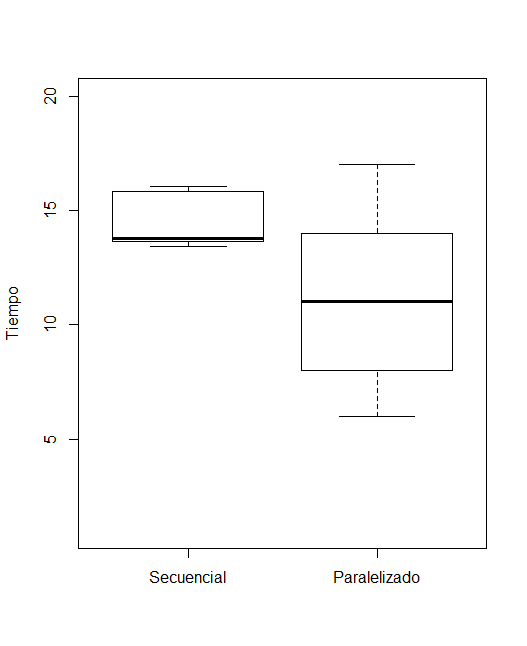
\includegraphics[width=80mm]{p8time.png}
\caption{comparación de tiempos}
\label{fig1}
\end{figure}


En la figura \ref{fig2} se puede observar que el tiempo es menor cuando se tiene una relación de \textit{k} y \textit{n} con los valores más bajos, las combinaciones de \textit{k} y \textit{n} se proporcionan en el cuadro \ref{combikn}.

\begin{figure}[h!]
\centering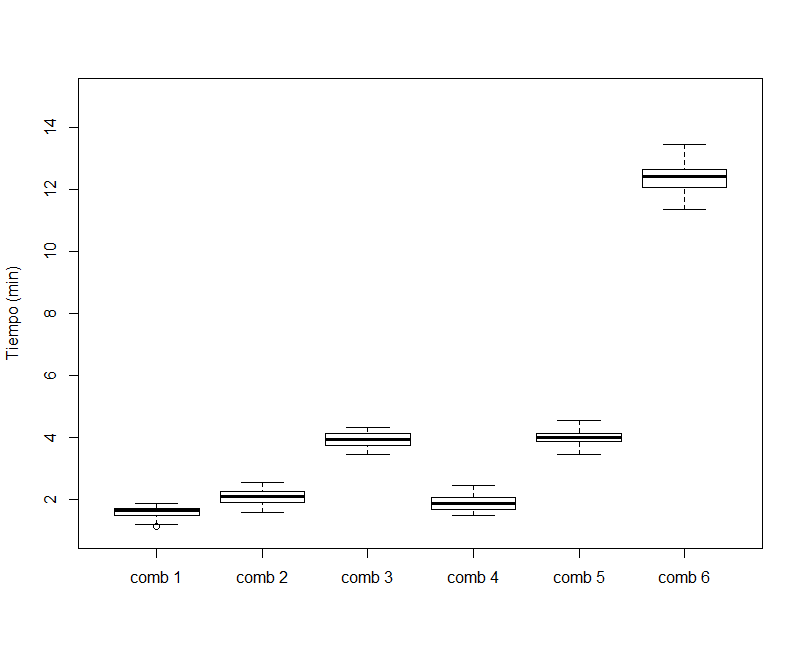
\includegraphics[width=100mm]{p8comb.png}
\caption{tiempo vs combinaciones de \textit{k} y \textit{n}}
\label{fig2}
\end{figure}

\begin{table}[h!]
\caption{Combinaciones de \textit{k} y \textit{n} }
\label{combikn}
\vspace*{3mm}
\centering
\begin{tabular}{c|c|c} 
Combinación&  \textit{k}  &  \textit{n} \\  \hline
1 & 1000 & 1000000  \\
2 &  1000& 10000000 \\
3 & 1000 &100000000\\
4 & 10000&1000000 \\
5& 10000&10000000\\
6 & 10000& 100000000\\
\end{tabular}
\end{table}

En la figura \ref{fig3} se observa la normalización del experimento paralelizado, cúmulos (\textit{k}) de 1000 y 10000 con las 3 combinaciones de \textit{n} correspondientes. Donde la relación de \textit{k} y \textit{n} con valores mayores dan una mejor normalización.

\begin{figure}[h!]
\centering
\subfigure[Paralelizado]{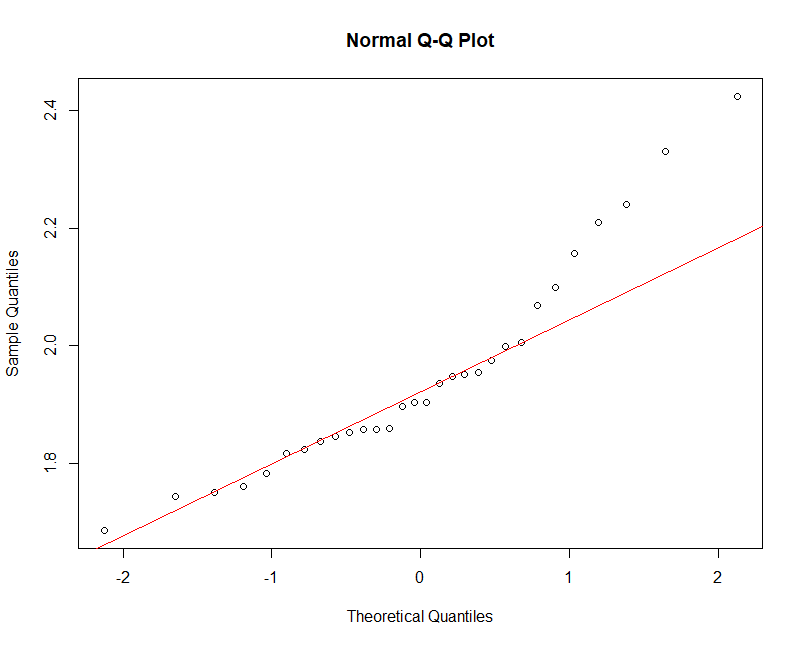
\includegraphics[width=60mm]{./paralelnorm.png}}
\subfigure[\textit{k} de 1000 con los 3 valores de \textit{n} ]{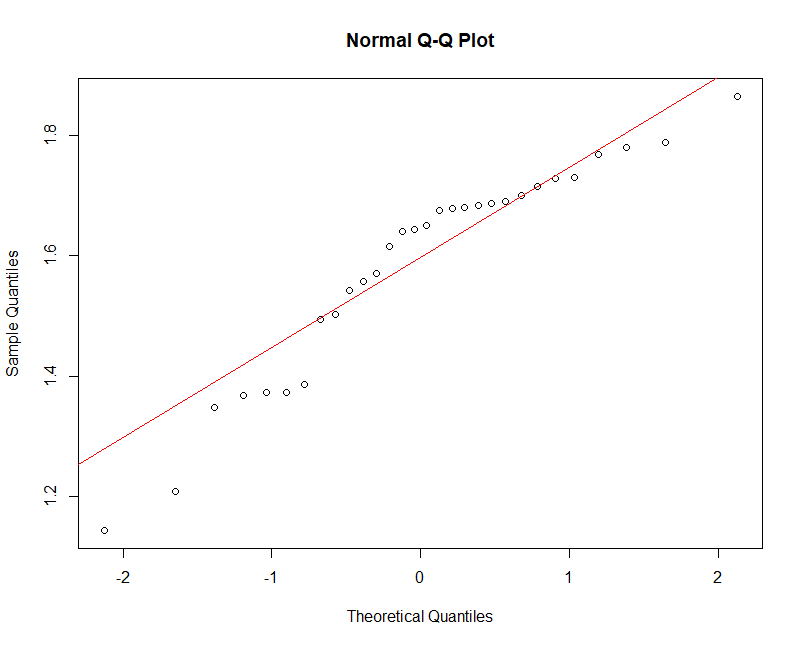
\includegraphics[width=60mm]{./normcomb1.png}}
\subfigure[\textit{k} de 10000 con los 3 valores de \textit{n}]{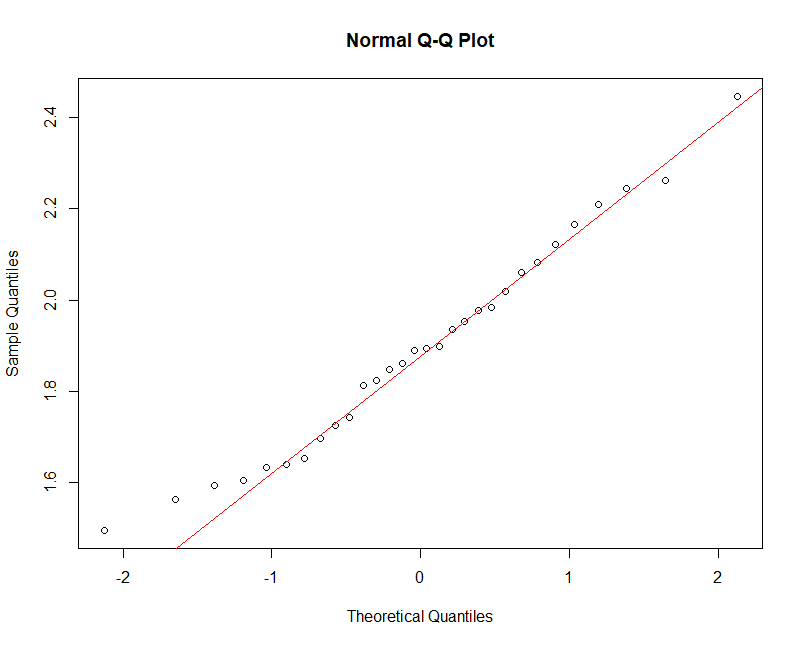
\includegraphics[width=60mm]{./normcomb2.png}}
\caption{Normalización de resultados} \label{fig3}
\end{figure}


\newpage
\section{Conclusiones}
Al tener una relación con valores de  \textit{k} y \textit{n} pequeños el tiempo es menor pero los valores no son muy significativos, no se normalizan, y al tener una relación de  \textit{k} y \textit{n} con valores grandes mejora la normalización pero el tiempo es mayor. Si se paraleliza el código aún más, se podrían obtener mejores tiempos al igual que un resultado más significativo.

\newpage

\title{Reto 1}
\section{Descripción}
Para el \textit{reto 1} se necesita saber en cuál paso los cúmulos son suficientemente grandes, usando los valores para \textit{k} y \textit{n} proporcionados por el código de la práctica \cite{elisaweb8} se obtienen los valores máximos de los cúmulos usando \texttt{max(cumulos)} y por medio de los histogramas se observan los pasos, se hacen 30 réplicas y se obtienen los datos estadísticos con \texttt{qqplot}.

\section{Resultados}
En la figura \ref{fig4} se observan los valores máximos de cúmulos normalizados y en la figura \ref{fig5} se puede observar que en el paso 3 hay mayor cantidad de cúmulos grandes que ya pueden filtrarse.

\begin{figure}[h!]
\centering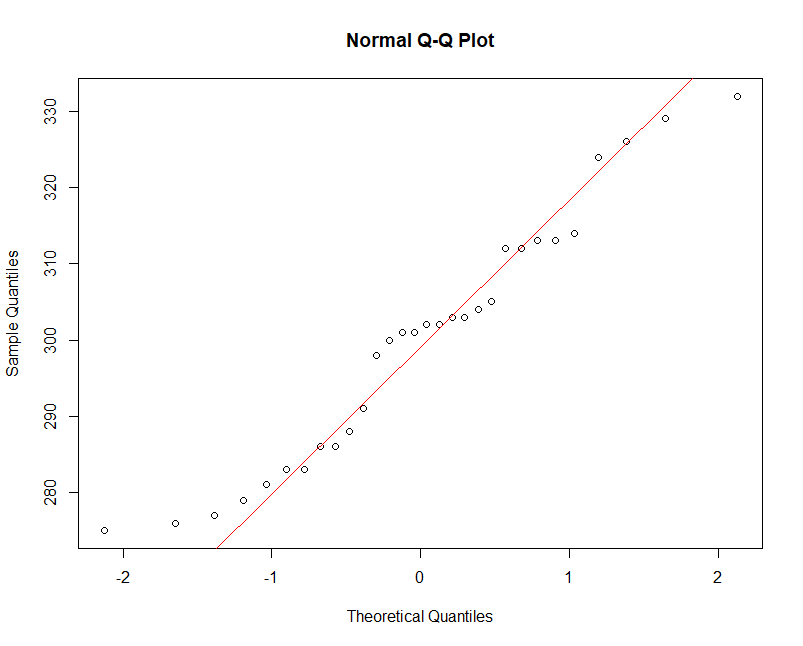
\includegraphics[width=80mm]{normfreqR1.png}
\caption{normalización de valores máximos de cúmulos}
\label{fig4}
\end{figure}

\begin{figure}[h!]
\centering
\subfigure[]{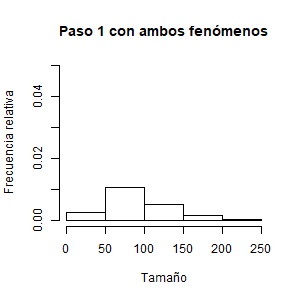
\includegraphics[width=60mm]{./p8R1.png}}
\subfigure[ ]{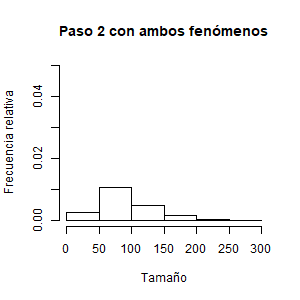
\includegraphics[width=60mm]{./p8R12.png}}
\subfigure[]{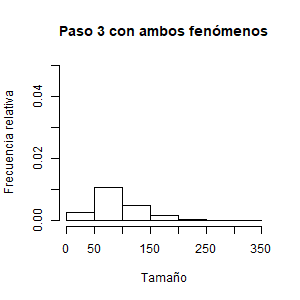
\includegraphics[width=60mm]{./p8R13.png}}
\subfigure[]{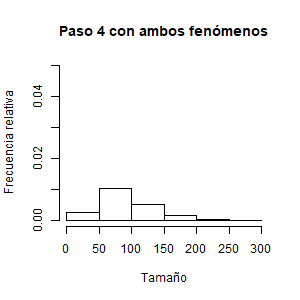
\includegraphics[width=60mm]{./p8R14.png}}
\subfigure[]{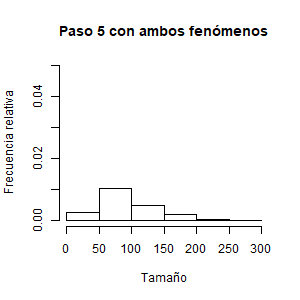
\includegraphics[width=60mm]{./p8R15.png}}
\caption{Histograma de pasos} (frecuencia vs tamaño de cúmulos) \label{fig5}
\end{figure}
\newpage
\title{Reto 2}
\section{Descripción}
Para determinar la importancia del valor de \textit{c} (valor crítico), en el código modificado para el \textit{Reto 1} se cambia su valor original dándole un valor de 40 y se grafica en una curva sigmoidal.

\section{Resultados}
En la figura \ref{fig6} se observa que al darle a \textit{c} un valor de 40, la probabilidad de que se formen cúmulos que ya no se rompan. En la figura \ref{fig7} se confirma en crecimiento de cúmulos a mayor cantidad de pasos.

\begin{figure}[h!]
\centering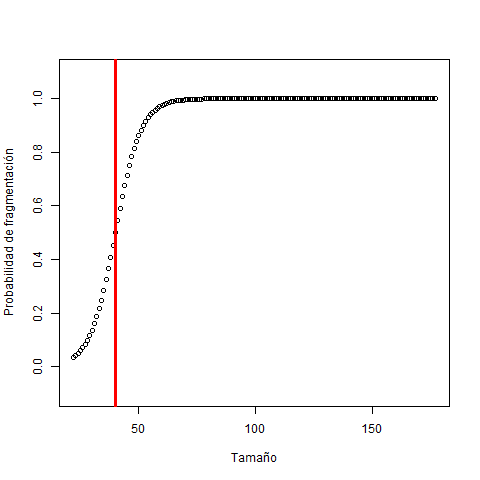
\includegraphics[width=80mm]{c40sigm.png}
\caption{Curva sigmoidal}
\label{fig6}
\end{figure}

\begin{figure}[h!]
\centering
\subfigure[]{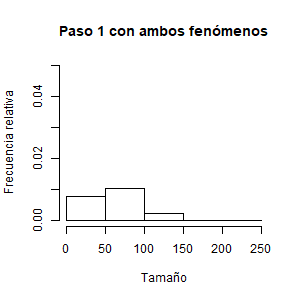
\includegraphics[width=40mm]{./c401.png}}
\subfigure[ ]{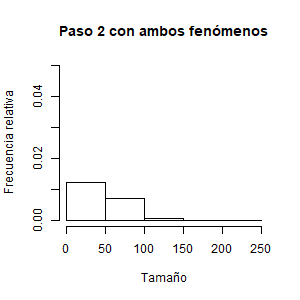
\includegraphics[width=40mm]{./c402.png}}
\subfigure[]{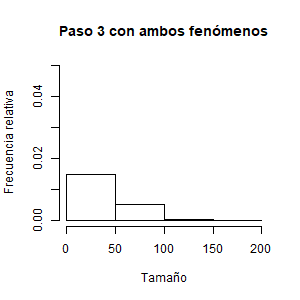
\includegraphics[width=40mm]{./c403.png}}
\subfigure[]{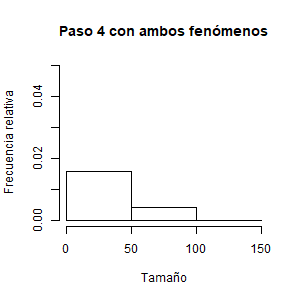
\includegraphics[width=40mm]{./c404.png}}
\subfigure[]{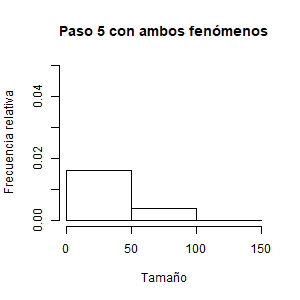
\includegraphics[width=40mm]{./c405.png}}
\caption{Histograma de pasos} (frecuencia vs tamaño de cúmulos) \label{fig7}
\end{figure}

\newpage
\section{Conclusiones}
El valor de \textit{c} afecta en la probabilidad de que los cúmulos se rompan o no, esto afecta en cuál paso se tendrán cúmulos de tamaño grande para poder filtrarlos y por lo tanto los tiempos varían también, por ejemplo, en este caso de \textit{c}=40, hay mayor probabilidad de que los cúmulos no se rompan, por lo que disminuirá el tiempo ya que no se tendrán que unir cúmulos rotos y se podrán filtrar más rápido.

\bibliographystyle{plainnat}
\bibliography{bibliosimu}

\end{document}